\section{Polialfabetici}

	\begin{frame}
		\begin{center}
			\LARGE{\textcolor{blue}{Cifrari a sostituzione polialfabetici}}
		\end{center}
	\end{frame}

	\subsection{Preliminari}
	
		\begin{frame}
			\frametitle{Idea}		
			\begin{itemize}
				\item Vogliamo \tblue{proteggerci} dall'analisi delle frequenze
				\item In generale vogliamo che due lettere uguali di ciphertext \tblue{non corrispondano} a due lettere uguali di plaintext
				\item Abbiamo bisogno di 
				\begin{itemize}
					\item \tblue{Un insieme} di cifrari monoalfabetici
					\item \tblue{Una regola} per decidere quale cifrario usare per ogni lettera del plaintext 
				\end{itemize}
			\end{itemize}
			\begin{columns}
				\begin{column}{0.2\textwidth}
					\begin{center}
						\begin{figure}
							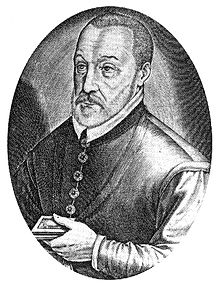
\includegraphics[width=\columnwidth]{img/Vigenere.jpg}
							\caption{Blaise de Vigenère}
						\end{figure}	
					\end{center}
				\end{column}
				\begin{column}{0.8\textwidth}
					\begin{itemize}
						\item Il più famoso cifrario di questo tipo è quello pubblicato nel 1586 dal crittografo francese \tblue{Blaise de Vigenère}
					\end{itemize}
				\end{column}
			\end{columns}
		\end{frame}
	
		\begin{frame}
			\frametitle{Il cifrario}		
			\begin{itemize}
				\item 26 caratteri alfabetici
				\item Sia \emph{m} la lunghezza della chiave $K$, $P_i,C_i,K_i$ la \emph{i-esima} lettera di plaintext, ciphertext e chiave. Per $i = 1,2,\dots$ le funzioni di encryption e decryption sono:
				$$E_K[P_i] = P_i + K_{(i-1\ mod\ m)+1} mod 26$$
				$$D_K[C_i] = C_i - K_{(i-1\ mod\ m)+1} mod 26$$
			\end{itemize}
			\begin{figure}
				\centering
				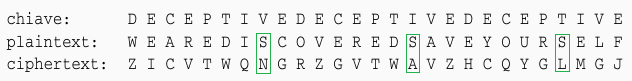
\includegraphics[scale = 0.6]{img/esempiovigenere}
				\caption{Esempio di cifratura}
			\end{figure}
		\end{frame}
		
		\begin{frame}
			\frametitle{Problema risolto? No!}		
			\begin{itemize}
				\item La \tblue{ripetizione} della chiave introduce \tblue{regolarità}
			\end{itemize}
			\begin{figure}
				\centering
				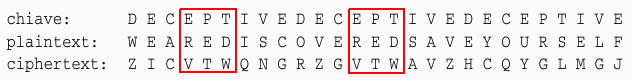
\includegraphics[scale = 0.5]{img/esempiovigeneredue}
			\end{figure}
			\begin{itemize}
				\item Vediamo come sfruttare questa \tblue{vulnerabilità}
			\end{itemize}
		\end{frame}
	
		{
			\setbeamercolor{background canvas}{bg=}
			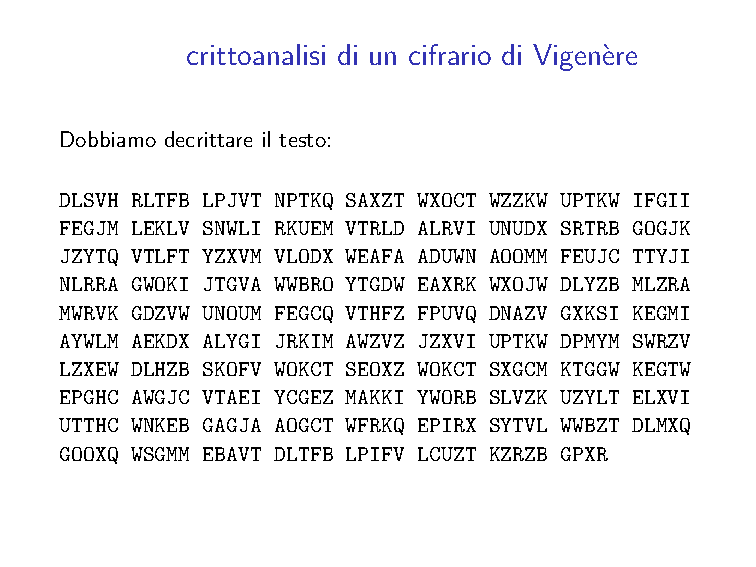
\includepdf[pages={1-3,5,9,11}]{esempi/vigenere.pdf}
		}
	
		\begin{frame}
			\frametitle{Verso One Time Pad}	
			\begin{itemize}
				\item Bisognerebbe poter utilizzare una chiave \tblue{casuale} e \tblue{molto lunga}, possibilmente, tanto quanto il messaggio da trasmettere $\Rightarrow$ \tblue{OneTime Pad}
			\end{itemize}
		\end{frame}